\documentclass[a4paper,12pt]{article}
\usepackage{graphicx}
\usepackage{titling}
\newcommand{\subtitle}[1]{%
  \posttitle{%
    \par\end{center}
    \begin{center}\large#1\end{center}
    \vskip0.5em}%
}

\title{Processing GeoSpatial Data in BaseX}
\subtitle{Master Thesis in fulfillment of the requirements for the degree of
Master of Science (M.Sc.)}

\author{\\\\Author: \\
	Masoumeh Seydi
	\\\\\\Supervisors: \\
	Prof. Dr. Marc H. Scholl \\ 
	Dr. Christian Gr{\"u}n \\
	\\\\\\
	Konstanz University}

\begin{document}
\maketitle
\thispagestyle{empty}

\newpage
\section*{Abstract}

\thispagestyle{empty}

\newpage
\section*{Acknowledgments}

\thispagestyle{empty}

\newpage
\tableofcontents

\thispagestyle{empty}
\newpage
\section{Introduction}
\setcounter{page}{1}

\subsection{Motivation}

\subsection{Overview}

\newpage
\section{GeoSpatial Data}

\subsection{GeoSpatial Data in Native XML Databases}

\subsection{General Spatial Requirements in NXD}
\newpage

\section{Related Works}
Here, we are going to summerize a large set of literature
over different XML handling methods. Section~\ref{storage} studies
different approaches to store GML. These approaches are investigated
with respect to the effectiveness storage models in terms of query processing.
  
\subsection{Storage}
\label{storage}
To store GML data more efficiently, \cite{Li2004} propsed an approach 
to store it in a spatial database. First the schema tree is generated
 and then it's mapped to relational schema to store all spatial objects as 
values of the mapped tables' field.  Spatial query can be submitted 
in XQuery-alike language with spatial functional extensions, and GML 
query is first translated into equivalent SQL query that is evaluated 
by spatial database management system.

\cite{Zhu2011} discussed another approach to store and query GML, 
focusing on non-schema documents.
First GML is parsed, the document tree is made. Then the nodes are analyzed and 
schema mapping is generated to store the doc in object-relational DB. 
Spatial and non-spatial queries are supported.

\cite{Zhang2008} Considering both characteristics of XML DB and GML spatial data, 
a native XML database based GML storage is proposed. A prototype system 
is developed, on the basics of JAXP (Java API for XML Processing) program API 
and JTS, containing schema mapping constructor, document storage tool, 
and spatial analyzer.

\subsection{Query Languages}
\label{index}
\cite{Fubao2010} XQuery language, recommended by W3C, is only 
applicable to non-spatial data. To query spatial data in GML, 
XQuery is expanded in data model, algebra, functions and operations, 
and formal semantics to achieve a GML query processor. The processor can 
deal with non-spatial and spatial queries, and the results will be outputted in GML.
Defined data types are: Geometry, Coord, Coordinates, Point, LineString, LinearRing, 
Polygon, Box, GeometryCollection, MultiPoint, MultiLineString, and MultiPolygon 
and spatial operations are: simple geometry operation, spatial relation 
operation, spatial analysis operation and specific geometry operation. 
JTS is called for handle operations

\cite{corcoles2001} Besides GML is used to represent and exchange 
the geographic data, it also benefits its XML-based model in interoperability, 
and more importantly, could be queried. In this study, the data model 
and algebra behind the language, based on a previously proposed model 
in which components and interrelations are represented as a directed graph. 
(The model includes new type of vertex for geometry types and its properties. 
Egdes represent elements containment, relationship between elements, and values.) 
With a data model and algebra, data types, and operation, the features that the language needs.

\cite{Lisa2006} Xquery is not a sutable language to query GML, 
since spatial related data types and semantics need to be treated different from XML. 
The purpose of this study is to define expand Xquery not for predefined GML elements, 
but more flexible.  A set of operators and functions on GML data types that cover 
the most typical queries over spatial data. The difference with the previous one is 
that this language is applicable not for predefined GML types, but to any type.

\cite{Chen2010} Integration of GML and Xquery. Adding spatial data types 
(Point, LineString, LinerRing, Polygon, MultiPoint, MultiLineString, MultiLinerRing 
and MultiPolygon) and spatial operation functions (basic, relational, analysis,.. functions), 
based on OGC Simple Features Specification for SQL, to XQuery can achieve GML spatial data query. 
Moreover to the previous studies in this subject GML spatial data query language 
based on XQuery, problem of GML spatial data query, reasons for extending XQuery to
support GML spatial data query, features of GML spatial data query language, 
content of XQuery spatial extension, architecture of GXQuery, implementation methods 
of GXQuery, and query examples of GXQuery were detially studied and discussed. 

\begin{verbatim}
FOR $var1 IN doc(“CDUTCampus.gml”)//Building,
$var2 IN doc(“CDUTCampus.gml”)//Building
WHERE $var1/gml:name/node() = “CDUT Palestra”
AND $var2/gml:name/node() = “CDUT Gymnasium”
RETURN geo:Contains(geo:Envelope($var1), $var2)
\end{verbatim}

\cite{Alemdros2013} A semantic version of Xpath language is defined, not based on the tree-based (syntactic) structure of the GML, based on the semantic structure of it.
A system is developed to store GML by PostGIS RDMS and then Xpath queries are translated into SQL, considering the GML schema. Fnaly, the result is represented in the system in KML.

\cite{Alemdros2011} A system developed that stores GML by means of PostGIS, and translates Xpath to SQL.
The results would be exported into KML to be visualized.

\cite{Gutierrez2004} A knowledge-based approach is used to querying heterogeneous spatial databases based on an ontology and conceptual and attribute similarities. The ontology, which may be independent of the databases, expands and filters a user query. Then, queries are translated into a formal specification of entity classes, which are compared against definitions in databases. This process is carried out by determining the conceptual similarity between entities in a user ontology and by comparing these entities in the ontology with entities in the conceptual models of databases. In addition, the specification of a query is done not only by identifying entity classes but also by considering constraints based on attribute values.

\cite{corcoles2004} Towards integrating spatial and non-spatial data, it's necessary to develop an integration sys. For querying the data in different sources. Here a prototype of a mediation system for querying XML spatial resources in GML is studied.  The main task of this approach is to provide users with a unique interface for querying spatial XML resources with different schemas, independently of their organization and location. It provides the infrastructure for formulating structured spatial queries by taking into consideration the conceptual representation of a specific domain in the form of an ontology. The resources are integrated using RDF. The most novel and critical feature of this approach is the querying of spatial XML resources, because it uses a different way from that of querying and relating non-spatial resources.

\cite{belussi2006} Base on the problem posed in different representation of spatial data in various resources ( For example, one dataset M1 may represent roads and bridges as regions, another dataset M2 may represent roads as regions and bridges as lines, a third dataset M3 may represent both as lines), or even in integration scenarios or architectures, a possible solution is to introduce some mechanism of query relaxation, by which approximated answers are returned to the user. In this study, the relaxation problem for spatial topological queries is considered. In particular,  some relaxed topological predicates are presented and is show in which application contexts they can be significantly used. In order to make such predicates effectively usable, the way that GQuery, an XML-based spatial query language, can be extended to support similarity-based queries through the proposed operators is also discussed.

\begin{verbatim}
Determine all roads overlapping some bridge.
for $x in document(bridge.xml), $y in document(road.xml)
where overlap($x/geometry, $y/geometry) = true
return $x

Determine all roads overlapping some bridge, up to a 22% error.
for $x in document(bridge.xml), $y in document(road.xml)
where overlapw($x/geometry, $y/geometry,R,L,0.22) = true
return $x 
\end{verbatim}

\cite{corcoles2003} An approach to integrate Geospatial data on the Web, storing them in GML, and using a query language. An ontology is used to solve the semantic heterogeneity of different GML documents.

\subsection{Indexing in famous XML databases}
\subsubsection{MongoDB}
\cite{mongogeneral2010}
\cite{mongoinaction2011}

Geospatial Index:

There is two special indexes in MongoDB: 2d indexes that uses planar geometry when returning results and 2sphere indexes that use spherical geometry to return results.

When an index is created, geohash values for coordinate pairs are calculated and then the geohashes are indexed.
Geohash is calculated by recursively dividing the a 2D map into quadrants and assigning each area a 2-bit value.


If the file contains just flat data, the 2d Index has to be used, but for those which also contain spherical data, 2sphere Index has to be chosen, since the distance function differs respectively.

Later on geohash values will be index using B-Tree. 
MongoDB also used B-Tree structure for other type of index, such as Single Field (e.g. indexing over names), Compound, Text Index. (Probably this point effect on the structure of geospatial index.)

Geospatial Functions:

geoWhithin, near (flat space), nearSphere (spherical space), geoIntersect, which could be mixed with other non-spatial functions (like find, ...). 
centerSphere (for spherical space), center (for flat space, define a circle with a specified radius), maxDistance (mixed with near functions to specify the demanded distance), box (defines a box, could be also mixed with geowithin function), polygon (defindes a polygon), inqueDocs (to prevent a through put a document twice in query results)

\begin{figure}
\centering
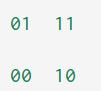
\includegraphics[width=0.5\textwidth]{mongoformat}
\caption{MongoDB format}
\label{fig1}
\end{figure}

mongoformat

Geohash (wikipedia)
Geohashes offer properties like arbitrary precision and the possibility of gradually removing characters from the end of the code to reduce its size (and gradually lose precision).
As a consequence of the gradual precision degradation, nearby places will often (but not always) present similar prefixes. Conversely, the longer a shared prefix is, the closer the two places are.
The main usages of Geohashes are
as a unique identifier.
represent point data e.g. in databases.
When used in a database, the structure of geohashed data has two advantages. First, data indexed by geohash will have all points for a given rectangular area in contiguous slices (the number of slices depends on the precision required and the presence of geohash "fault lines"). This is especially useful in database systems where queries on a single index are much easier or faster than multiple-index queries. Second, this index structure can be used for a quick-and-dirty proximity search - the closest points are often among the closest geohashes.
One limitation of the Geohash algorithm is in attempting to utilize it to find points in proximity to each other based on a common prefix. Edge case locations close to each other but on opposite sides of the Equator or a meridian can result in Geohash codes with no common prefix.[1]
Secondly a geohash essentially defines a bounding box within which a location lies, therefore two locations may be spatially very close but have different geohashes. In order to be useful to proximity searches, the surrounding eight geohashes of a geohash must be calculated and the locations matching these pulled out, therefore complicating potential usage in proximity searches.

\subsubsection{MarkLogic}
Geospatial data is marked up in XML elements and/or attributes. MarkLogic could handle and query different formats, such as GML, KML, GeoRss, and even general format for geometric data which are not based on a specified format. Only WGS84 and Raw coordinate systems are supported. WGS84 is used for data on the earth geometry, and raw coordinate system is suitable for data on flat plane.

Regarding the geospatial queries, the following types are supported:
\begin{itemize}
\item point query--matches a single point
\item box query--any point within a rectangular box
\item radius query--any point within a specified distance around a point
\item polygon query--any point within a specified n-sided polygon
\end{itemize}

Additionally, there are some Geospatial Operations as built-in functions to perform operations on geospatial data (in cts namepsace):

 box-intersects → Returns true if the box intersects with a region.
 circle-intersects → Returns true if the circle intersects with a region.
 polygon-intersects → Returns true if the polygon intersects with a region.
 complex-polygon-intersects → Returns true if the complex-polygon intersects with a region.
 polygon-contains → Returns true if the polygon contains a region.
 complex-polygon-contains → Returns true if the complex-polygon contains a region.
 distance → Returns the distance (in miles) between two points.
 shortest-distance → Returns the great circle distance (in miles) between a point and an region. The region is defined by a region.
 destination → Returns the point at the given distance (in miles) along the given bearing (in radians) from the starting point.


 XQuery Primitive Types And Constructors
These constructors (as functions from search module, cts namespace) are used in geospatial queries (cts:query constructors), defining regions as instances of cts:region, then the query returns true if the searching data are inside the region.
 cts:box 
 cts:circle
 cts:complex-polygon
 cts:linestring
 cts:point
 cts:polygon

 WKT

	WKT language also is supported for geospatial data representation. The parse-wkt function is used when WKT is used. It converts WKT to sequence of region items. Also, cts:to-wkt function could convert cts:region type in MarkLogic to WKT.

GeoSpatial Coordinates and Regions in MarkLogic Server


Latitudes and longitude pairs shape point. Points shape other geometries, like circle or polygon. Boxes are formed by 4 points which on the surface of the Earth, the edges of the box are arcs, but when those arcs are projected into a plane, they become two-dimensional latitude and longitude lines, and the space defined by those lines forms a rectangle.


The Geospatial Index
It is not based on quad or R-tree. It works like a range index with points as data values. In this range index, every value is a pair of latitude and longitude. Like an array of x,y values, sorted mainly based on lat and then long values. The values in array also are connected to the corresponding doc.
The points would be founded easily in a sorted structure. Boxes could be found first by finding the lat range, then checking for the long range. For circles and polygon as more complex ones, the bounding box is used to find the region they belong to. Also, to check if a point is inside the polygon, the number of intersections with the northward or southward arc of the point is counted. 

…. 

Different types of Geospatial Indexes: (???)

 Geospatial Element Indexes: data is represented by whitespace or punctuation separated element content 
 Geospatial Element Child Indexes: data comes from whitespace or punctuation separated element content, but only for elements that are a specific child of a specific element.
 Geospatial Element Pair Indexes: data comes from a specific pair of elements that are a child of another specific element.
 Geospatial Attribute Pair Indexes: data comes from a pair of specific attributes of a specific element.
 Geospatial Path Range Indexes: data is expressed in the same manner as a geospatial element index and the element or attribute index is defined by a path expression.


Geospatial Index Positions
	For each geispatial index there is a positions options, which is used for queries with restrictions 	of data distance inside the document.

Geospatial Lexicons1
Provided by spatial index, containing unique values of  geospatial data. 

“geo” Xquery Library
geo:box
Create a cts:point value from an element representing a box in one of the supported markup vocabularies.
geo:circle
Create a cts:circle value from a radius and an element representing a point in one of the supported markup vocabularies.
geo:geospatial-query
Returns a cts:query matching points within given regions.
geo:geospatial-query-from-elements
Returns a cts:query matching points within given regions.
geo:interior-polygon
Create a sequence of cts:polygon values from a polygon element in one of the supported markup vocabularies.
geo:point
Create a cts:point value from an element representing a point in one of the supported markup vocabularies.
geo:polygon
Create a cts:polygon value from a sequence of point elements in one of the supported markup vocabularies.


“gml” Xquery Library
gml:box
Create a cts:box value from a GML Envelope element.
gml:circle
Create a cts:circle value from a radius and GML Point element.
gml:geospatial-query
Returns a cts:query matching points within given regions.
gml:geospatial-query-from-elements
Returns a cts:query matching points within given regions.
gml:interior-polygon
Create a sequence of cts:polygon values from a GML Polygon element.
gml:point
Create a cts:point value from a GML Point element.
gml:polygon
Create a cts:polygon value from a sequence of GML Point elements or a GML Polygon element.


“geoRss” Xquery Library
georss:circle
Create a cts:circle value from a radius and GeoRSS point element.
georss:geospatial-query
Returns a cts:query matching points within given regions.
georss:point
Create a cts:point value from a GeoRSS point element.

“kml” Xquery Library
kml:box
Create a cts:point value from a KML LatLongBox element.
kml:circle
Create a cts:circle value from a radius and KML Point or Location element.
kml:geospatial-query
Returns a cts:query matching points within given regions.
kml:geospatial-query-from-elements
Returns a cts:query matching points within given regions.
kml:interior-polygon
Create a sequence of cts:polygon values from a KML Polygon element.
kml:point
Create a cts:point value from a KML Point or Location element.
kml:polygon
Create a cts:polygon value from a KML polygon or a sequence of KML Point or Location elements.


“cts” Functions
Part of these functions also contain geospatial function: 1 2
----------------------------------------------------------------------------------------------------------------------------
For querying on geospatial data, after loading the data into the DB and making the indexes, primitive types should be constructed to be used in the geospatial cts:query functions. Then, geospatial queries needs to be constructed, using primitive types. 
Also, there are modules to convert the Metacarta, GML, KML, and GeoRSS formats to cts:box, cts:circle, cts:point, and cts:polygon formats, to pass them into the cts:query constructors and make appropriate queries.

\subsubsection{eXist-db}
The design if spatial index in eXist-db doesn't store character data from the document. It stores WKB index entries in a JDBC database, namely a HSQLDB. In other words, the spatial data is stored in the DB, but geometries, as JTS Geometry instances, are held in memory, waiting for a special mode to be flushed into a relational DB, insertion or removal. The Geometry WKT would be serialized and deserialized to and from the database.
The index is made by the relational db (uses an SQL database to index spatial data) and the geometric functions are applied using JTS library.



Both PostGIS and Oracle Spatial share the same “R-Tree” [1] spatial index structure. R-Trees break up data into rectangles, and sub-rectangles, and sub-sub rectangles, etc. It is a self-tuning index structure that automatically handles variable data density and object size.

Ideas

Query general format geospatial data, considering the data as a set of points, ...
Storing the eospatial data in geohash ???
…


\subsection{Others}

\newpage

\section{GeoSpatial Indexing}
According to \cite{survey}, indexing would dramatically influence efficient data manipulation and storage. Like any other type of data, Geo Spatial data would be needed o be indexed. Conventional index types are not suitable to support the spatial data, since the spatial data is very large and complex in structure and relations. Also, the operators used for data retrieval are complicated and spatial orderings would be hard to define. Another point which makes the traditional indices not suitable for spatial objects is that they would consider the spatial objects in one dimension and do not preserve the spatial proximity.

As it is examined in \cite{survey}, a large number of spatial indexes has been introduced to improve the spatial data retrieval.
The strength or weekness of an indexing approach mostly depends on requirements, query types, and applications. In the following sections, we go through selective spatial indexes based on three data structures Binary-tree, B-tree, and Quad-tree.

\subsection{Binary-tree Based}
The indexes in this group are basically and conceptually derived from the binary search tree. They adopt and generalize the idea of partitioning the space. Here some of them are explained.

\subsubsection{The kd-Tree}
This index, which was first introduced by Bentley \cite{bently1975}, is a binary search tree structure for organizing k-dimensional points. As it is explained in \cite{bently1975}, the basic idea is alternatively split the area by x- and y-coordinate, that at each level splits the points half in left, half in right, half below, and half above respectively. For every non-leaf node, there is a k-th dimension discriminator, which defines the the left and right subtrees order association with this node. If the discriminator is associated to the i-th dimension, all the i-th attribute of the sub-nodes in left subtrees are smaller than this node, and all the right sub-tree nodes have the i-th attribute greater.

\begin{figure}
\centering
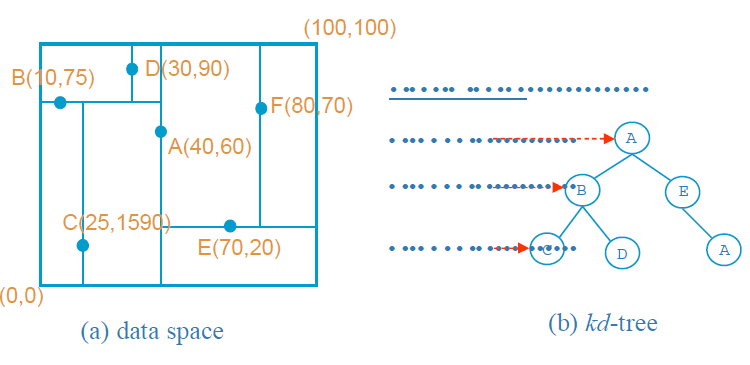
\includegraphics[width=\textwidth]{kdtree}
\caption{kd-tree}
\label{fig1}
\end{figure}


When an item is deleted, a node from the sub-tree must be replaced. Here arises a complication that based on the discriminator in that level, let's call it i, either the node with the smallest i in right sub-tree should be replace or  the node with the biggest i in left sub-tree. A non-homogeneous kd-tree was proposed to make this process cheaper. 
Kd-Tree has been used a lot in intensive searches, but some variants has been introduced to make a better performance in clustering, searching, storage efficiency and balancing [survay], such as …..
and below we discuss some of them.

Main memory storage of the index trees are mostly a problem, since it is too big to be placed there  [survay]. Hence, the storage has to be done into disk space. Using binary search tree paging techniques [CeS82 survay] or tree organization of B-trees [BaM72 survay] to store the kd-Tree proposes new indexing structures.

Using properties of both kd-tree and B-tree [reference], the KDB-tree rebuilds the kd-tree to improve some inefficiencies of it.  It means benefits of the balanced kd-trees and the I/O efficiency of B-trees are together. It uses the disk space to bring the kd-tree on disk. 

The method which is used to build  KDB-tree is a space partitioning structure such that the partitions do not overlap each other. The partitions which stand for pages as organizational units, are organized in k-d-tree structure. 
KDB-tree has two basic structures: region page, consist of (region, pageID) pairs, and point page, consist of  (point, pageID) pairs. The region page contains the description of its subpages and a reference to those pages. The point pages contains actual data and references to them. 

\begin{figure}
\centering
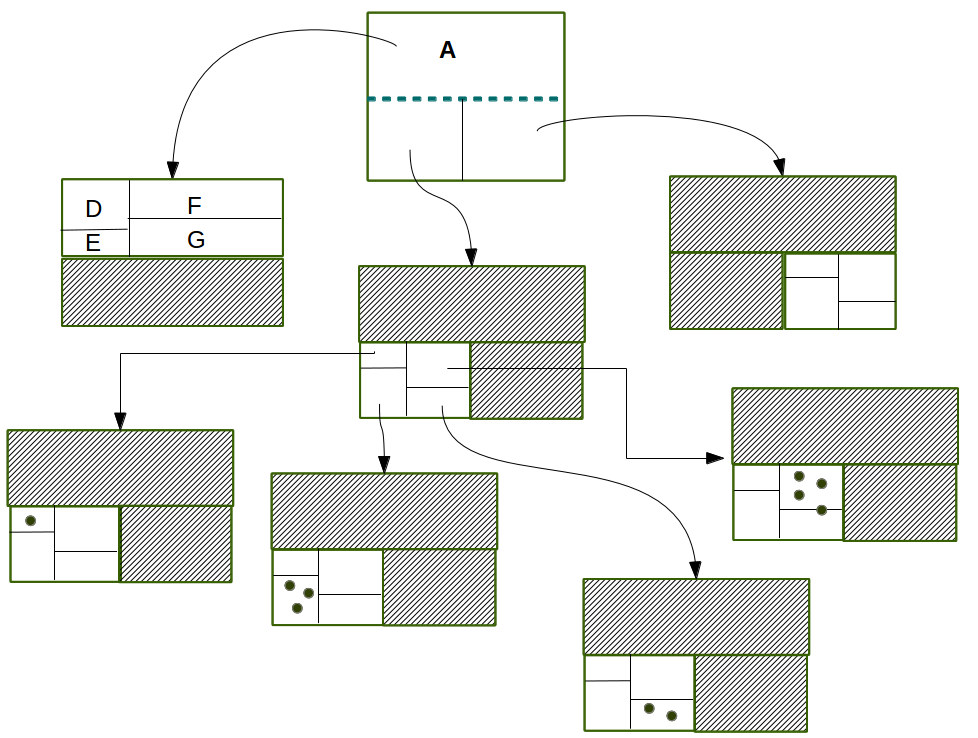
\includegraphics[width=\textwidth]{kdbtree}
\caption{kdb-tree}
\label{fig1}
\end{figure}

The pagination of the B-tree is integrated in the KDB-tree and consequently the tree is height-balanced. Space utilization and efficiency might be low or high, though, since the downward propagation of splitting, caused by region split, may cause low storage utilization. On the other side, there is no guarantee for minimum space utilization. Since partitions do not overlap, it is not always easy to find disjoint partitions to divide a region. So, those partitions must be split at the same value as parent, even though they do not use the minimum amount of space specified for each node. By this problem the range queries' performance is poor. 

Another variation of KDB-Tree which can be distinguished by two features: …
Since in a the region split in lower levels result in sparse nodes, hB-Tree (the holey brick Btree) as a multi-attribute index structure is proposed. Data spaces could be holey. It allows the data space associated with a node to be non-rectangular and it uses kd-trees for space representation in its internal nodes. The leaf nodes are known as data nodes and the internal node as index nodes. An index node data space is a union of its child node subspaces which are obtained through kd-tree recursive partitioning. It is height balanced since it is based on the K-D-B-Tree. 
Advantages of this structure is removing the sparse nodes of the K-D-B-Tree and reduction of search time and space utilization, since kd-tree is used. 
Disadvantages of this structure is that the deletion and splitting of nodes are expensive and also multiple references to a data node will lead to more than one traversal of a path.

\begin{figure}
\centering
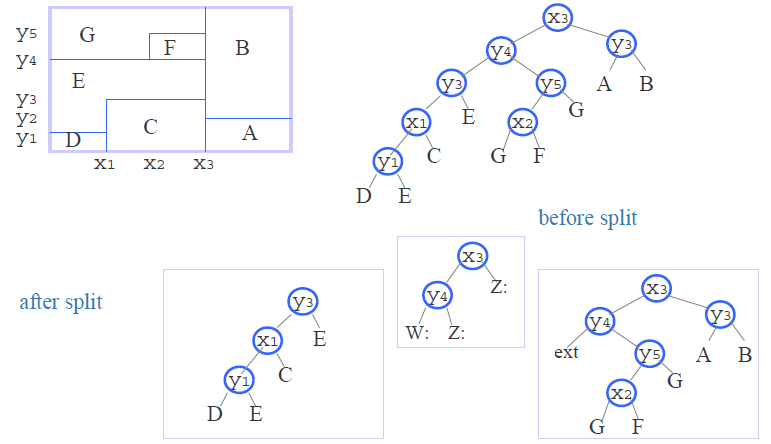
\includegraphics[width=\textwidth]{hbtree}
\caption{hb-tree}
\label{fig1}
\end{figure}

\subsubsection{Matsuyama’s kd-Tree}
This structure is introduced for non-point objects and an extensive duplication strategy is used. The directory is a kd-Tree and a data page is associated for each leaf and those objects which overlaps multiple data spaces are identified in data page and also duplicates. Hence, the data page contains identifiers of the objects totally or partially contained in the corresponding data space.
The point is that this structure is not suitable for large objects since duplication and redundant storage of objects would result in high overhead.

\subsubsection{4D-tree}
Indexes rectangular objects using kd-tree by mapping the objects into points in a four-dimensional space. Each 2D rectangle with (x1, y1) and (x2, y2) is considered as a 4D (x1, y1, x2, y2). As kd-tree the discriminators are chosen cyclically from this set. For each node, a discriminator, discriminator value and pointers to two children are stored. 
For a region search (qx 1, qx 2, qy 1, qy 2), depending on the discriminator, one of the x1 <= qx2, x2  >=  qx1, y1 <= qy2 or y2 >= qy1 has to be done to determine which subtree (or both) has to be searched.
The major problem associated with the 4-d-tree is its intersection search, which can be very costly due to the need for traversal of both subtrees when a query region lies in a subspace that cannot not bounded tightly using the discriminator values.

\subsubsection{skd-tree}
The spatial kd-Tree alters the kd-tree in a way that objects are indexed by their centroid and the minimum bounding box of the object is also stored in the node. This structure is suitable for non-point spatial objects. In a kd-tree the objects which are contained in more than one space, will be referenced more than once. To avoid the duplication virtual subspaces are defined which include the original subspaces. So, each object are placed in the subspace based on its centroid.
With this devision, we just need one more value for each subspace which shows min/max values along the dimension of the discriminator. Therefore, the structure of each node would consist of:
Two children
The discriminator and it's value
The max/ min value of objects left(LOSON)/right(HISON) subspaces along with dimension of the discriminator
The maximum/minimum value of LOSON/HISON the nearest virtual line which bounds the data whose centroid are inside the LOSON/HISON.

\begin{figure}
\centering
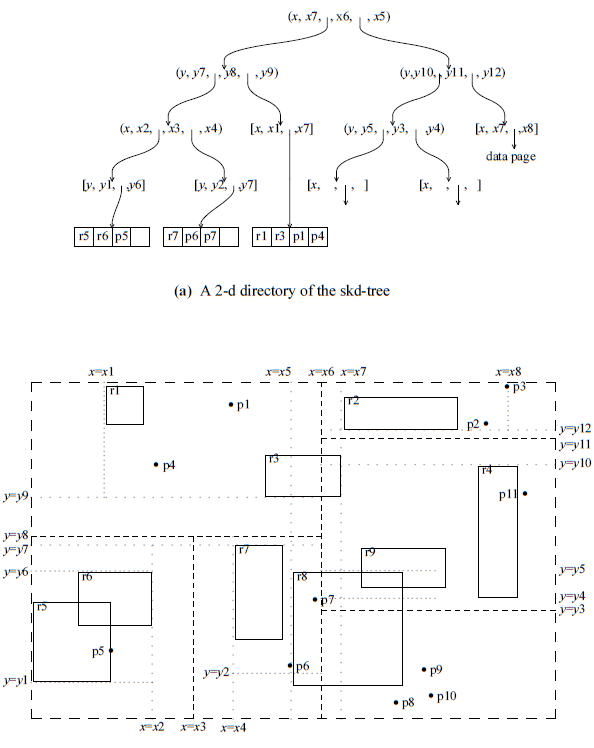
\includegraphics[width=\textwidth]{skdtree}
\caption{skd-tree}
\label{fig1}
\end{figure}

During traversal a rectangular space is associated with each node and materialized  such that is tested against the query region if it intersects the region. 
(Since the virtual boundary may sometimes bound the objects tighter than the partitioning line, the intersection search takes advantage of the existing virtual boundary to prune the search space efficiently. To further exploit the virtual boundaries, containment search which retrieves all spatial objects contained in a given query rectangle was proposed. During tree traversal, the algorithm always selects the boundaries that yield smaller search space. The direct support of containment search is useful to operators like within and contain. The search rapidly eliminates all objects that are not totally contained in the query region.)
The Sdk-tree is memory-based, not a disk-based, data structure, thus is not suitable for very large databases.

\subsection{B-tree based Indexing Technique}
\subsubsection{R-tree}

Minimization of both coverage and overlap is crucial to the performance of R-trees.
\subsubsection{$R^*$-tree}
The $R^*$-tree is found to be more efficient than some other variants, and the R-tree using linear splitting algorithm is substantially less efficient than the one with quadratic splitting algorithm. In general, the R*-tree is an improvement over the R-tree at the expense of more expensive insertion.

This structure tries to reduce overlaps between directory rectangles and the area covered by a rectangle, in order to make better performance, since minimum overlaps leads to less number of branches to be traversed in queries and minimum coverage helps to decide on the paths to traverse on higher levels. 
R*-Tree does these optimizations with revised node split and also forced insertion which finds a better place for a node that its original place. In R-Tree insertion-build structure is highly suboptimal and insertion and deletion could improves the R-Tree dramatically.
 (Using the idea of reinsertion of the R-tree, Beckmann et al proposed a reinsertion algorithm when a node overflows. The reinsertion sorts the entries in decreasing order of the distance between the centroids of the rectangle and the covering rectangle and reinserts the first p (variable for tuning) entries. In some cases, the entries are reinserted back into the same node and hence a split is eventually necessary. The reinsertion will no doubt increase the storage utilization; but it can be fairly expensive when the tree is large. The R*-tree is found to be more efficient than some other variants, and the R-tree using linear splitting algorithm is substantially less efficient than the one with quadratic splitting algorithm. In general, the R*-tree is an improvement over the R-tree at the expense of more expensive insertion.)

\subsubsection{The Buddy Tree}
(In comparison to previously proposed tree structures such as the K-D-B-tree, the buddy-tree guarantees a more efficient dynamic behavior.Moreover, indirect splits which cause low storage utilization and high insertion costs in the K-D-B-tree, are completely avoided. This structure is 
It avoids the downward splitting of the K-DB-tree, the overlapping problem of the R-tree and the dependency of structures upon the insertion of data. The buddy-tree generalizes the buddy system of the grid-file to organize correlated data efficiently, by bounding the data points tightly using the bounding rectangle concepts of the R-tree and organize the directory as in the R-tree. Like grid-files, the non-zero sized data have to be mapped into higher dimension.
An important feature of the buddy-tree is that it does not partition empty data space. Therefore queries, such as partial match queries, where the query region intersects with empty data space, can be performed much faster than by conventional structures partitioning the complete data space.
The following summarizes the design properties of the buddy-tree:
empty data space is not partitioned
insertion and deletion of a record is restricted to
exactly one path
no overflow pages
directory grows linear in the number of records
performance is basicly independent of the sequence of
insertions
efficient behavior for insertions and deletions
very high fan out of the directory nodes)

\subsubsection{The Packed R-Tree}

In order to minimize storage space, coverages and overlaps in R-Tree, constructing a static tree is proposed. To make this tree, first the objects are ordered along a coordinate. The object with the minimum value then is chosen to find the M nearest objects to that one, and assigns them to a node. Here M is the maximum number of objects that are allowed in a page. This step is repeated until the whole objects are assigned to a node. The bounding box of the leaf nodes are higher level objects. These are also ordered and assigned to the nodes. The process repeats until the number of the remained nodes is less than M. If so, they are assigned to the root.
The main objective of the algorithm is to reduce the storage space, the coverage and overlap of rectangles, in order to improve the search efficiency.

\subsubsection{R+-Tree}

This structure is a compromise between the R-tree and the K-D-B-tree, to solve the overlapping problem of covering rectangles. It has just some difference:

Nodes of an R+-tree are not guaranteed to be at least half filled.
 The entries of any intermediate (internal) node do not overlap.
 An object identifier may be stored in more than one leaf node.

The duplication of the objects in the tree avoids overlappings and consequently leads to less path traversals in point queries. 
On the other hand there is some disadvantages: it might be bigger that R-Tree as a result of duplications, and the construction and maintenance are more complex that R-Tree or other variants. 
Also, in insertion cases into the tree a case would happen that the	covering rectangles of some entries can prevent each other from expanding to include the new object. In other words, some space ("dead space") within the current node cannot be covered by any of the covering rectangles of the entries in the node. If the new object occupies such a region, it cannot be fully covered by the entries. When a new object cannot be fully covered, one or more of the covering rectangles are split. This means that the split may cause the children of the entries to be split as well, which may further degrade the storage efficiency.
In performance study, in the comparison between R-trees and R+-trees, it is found that the R+-tree requires much more splits, especially for large data objects, but lesser splits for smaller data objects. 
In general, the query efficiency tests show that R+-trees perform better for smaller objects and slightly worse off for larger objects.

\subsubsection{STR-tree}

\subsubsection{Cell-tree}
The cell tree introduces a structure to overcome the overlapping bounding rectangle problems of R-trees and the "dead space" (empty space) problems of R+-trees. Partitioning is done in a recursive way, but not necessarily with rectangles. Instead, the regions are polyhedral, as bounding polygons. Subspaces do not overlap.  
\begin{figure}
\centering
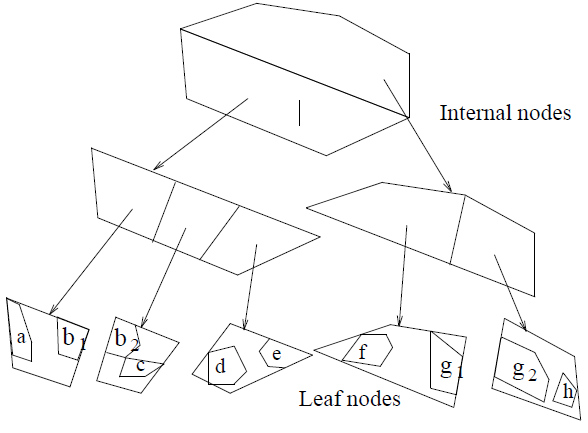
\includegraphics[width=\textwidth]{celltree}
\caption{cell-tree}
\label{fig1}
\end{figure}

Like R+-Tree, objects might be represented in more than one leaf node. One problem with such an instruction which duplicates the objects is that each new object may be divided into multiple pieces in order to store them in a tree where internal node bounding polygons do not overlap. Specially in populated DBs. 
(Each split of a node leads to a decrease in the node data space but to an increase in the number of nodes per object. To overcome the fragmentation and duplication problems, Gunther and Noltemeier proposed to store oversized objects which may greatly increase the number of object identifiers being stored in the leaf nodes in separate "oversize shelves". These oversize shelves are data nodes linked to internal nodes in the cell-tree, in one way, causing the tree to be not height-balanced. The placement of a new object in the subtree or oversize shelf requires some optimization. The oversize page shelf can be overflowed and a split on this shelf is necessary.)
\subsubsection{Quadtree}
It is organized in a way similar to the region quad-tree. A region is recursively partitioned until the resulting quadrants do not contain any rectangle. During the subdivision, all rectangles that intersect with either of the two partitioning lines are associated with the partitioning lines. The rectangles that are associated with a quadrant must not belong to any ancestor quadrant. It is assumed that no two rectangles overlap.

\newpage

\section{Spatial Query in BaseX}
\subsection{Geo Module in BaseX}

Geo features in BaseX are implemented based on the EXPath Geo Module Specification [ref.]. The module comprises a set of functions, widely used in geographic and geometric analysis, such as intersection, within, distance, boundary, centroid, diference, union, and etc. The functions are implemented in Geo module, mainly added to the “basex-api” package in BaseX. In addition, spatial index structure is implemented in BaseX core. Geo module is an individual package with a set of classes as below,
Geo
GeoError
GeoTest
GmlReader
GeoIndex

Geo class is the main one, in which all geo spatial functions are defined and implemented and could be used in Xquery. GeoErrors defined error functions with related massages to be thrown. GeoTest class contains functions to test the module. Functions required to read the GML geometries as xml elements are implemented in GmlReader class.  GeoIndex class offers functions to use geo spatial index in geo functions and queries. Spatial indexing and related implementation details will be described in he next section. Here we explain general functionalities of this module.
The geometries supported in this module, based on GML 2.0 standard, are,
Point
LineString
Polygon
Multi.. ???

The geo functions in Geo.java class are the public ones, accessible from BaseX GUI, using some private functions of the class to read geometries or write them out into the GUI. Besides, each function uses corresponding function from JTS library[ref.] to do the required geometric operation and provide the geo spatial functionalities. Here we briefly explain the process when input geometries either from a variable or a database node is processed and the result is returned.
Let's start it with an example, asking for geometries (here just the polygons are mentioned) within a specified polygon (p). The query should be written using Xquery via BaseX GUI as follow,

\begin{verbatim}
let $p := 
<gml:Polygon>
  <gml:outerBoundaryIs>… </gml:outerBoundaryIs>
<gml:Polygon>
	
for $x in //gml:Polygon
  return if ( within($x, $p) ) then $x else ()
\end{verbatim}

Each geo spatial function has at least one geometry as an input, as function “within” above. As in the example, the $p variable is provided as a node and the $x variables are database nodes. To read the geometries as a node, when the geo function (within) is called, the private function “geo” first checks the element name to make sure that at least the node name is a valid geometry name. It means, if the element name is something out of the set of geometry names, the function would throw an error. 
Then, the gmlReader class is used to read and pars the element and to check their validity based on GML2.0 format. The reader is implemented as the class “GMLReader” and differently reads the elements based on their types (tag names). If the element is a valid GML geometry, the function create the corresponding geometry, using JTS constructors. Otherwise, an appropriate error massage will be thrown. For instance, if a polygon does not have any outer ring or the coordinates of a geometry are not valid coordinates. 

(Figure for this process)

Now, the geometry is ready to be input for an geometric operation. For example, to check two geometries whether they intersect each other, the symmetric distance of two geometries, and number of inner rings of a polygon. The operation is done using the JTS function. The results could be numbers, boolean values, geometries, string, and few other data types. In case which the output is geometry, it needs to be converted to a database node (DBNode). Therefore, first JTS gml writer class is used to convert the GML format of the geometry to string. Next, the string, is used to create database instance to form a database node. Finally, the output is shown on GUI. This steps are shown in Figure ….

\subsection{Geo Module Limitations}
Geo functions are perfectly working, but the point is that the performance is not satisfying, when the  data needs to be queried. A point that makes this problem more serious is that the geo spatial data have commonly huge size. This brings the idea of indexing, designed based on the geo spatial requirements.
The first point to consider related to performance issue is that the whole database is processed for every type of query. It means, in some queries checking parts of the file and a range of geometries would be enough to get the result. For example, if we want to find the intersecting geometries of a specific geometry, there is no need to check the whole geometries and examining the area near and around to this geometry would be enough to get the results. This comes from the characteristic of the spatial data. That means, the data file is in fact written form of the geometries which are positioned in space. 
This idea would help to use an indexing structure for such a queries and decrease the number of scanned geometries and therefore, better timing.
As it is explained in related work [??], there are different spatial indexing structure. The one that we use is JTS STRTree. STRTree has the basic structure of the R-Tree, with the improved performance in comparison to R-Tree [??]. This structure is once made, when the spatial index for a database is requested, then uses two step filtering for each time a query needs to be done. It should be considered that only specific queries would benefit from this index,
intersects
within
contain
relates 
overlaps
crosses
touches
equals
disjoint*

The tree structure, holding the bounding boxes in inner nodes and geometries in leaves, is written into a file and each time the index is applied, the file is read into main memory (see Figure ???). The first step of filtering is to select those nodes of the tree, which intersect with the given geometry's bounding box. And in the second step, the geometric operation is applied on geometries inside the selected areas, whether they meet the query condition. This strategy will dramatically decrease the number of processes in database. In the following sections we represent the performance issues of the index structure.


\subsection{Geo Spatial Index in BaseX}
Spatial index in BaseX is added both in baseX core and also BaseX-API packages. The main structure of the index is added as a package in core, defining the index builder classes, based on the core structure of BaseX. The class “SpatialBuilder” extends “IndexBuilder” and builds the index tree using pre-values of the nodes and serializes it into the disk, using JTS serializer. In the end, a file called “STRTreeIndex” for the related database is created. 
The other GeoIndex class in BaseX-API extends QueryModule and implements the methods defined by JTS STRTree class for reading the index file from hard disk into memory and filtering. These functions could be combined with regular geo functions, when spatial index is created for a database, to have the benefit of filtering feature and gain better performance. The below example clarifies how the indexing function should be used,
\begin{verbatim}
import module namespace geo-index = "http://expath.org/ns/GeoIndex";
import module namespace geo = "http://expath.org/ns/Geo";
declare namespace gml="http://www.opengis.net/gml";
let $a:= <gml:Polygon>
              <gml:outerBoundaryIs>
                	<gml:LinearRing> 
			<gml:coordinates>3.9,50.6 6,52.8 4.5,52.8 3.9,50.6</gml:coordinates> 
		</gml:LinearRing>
              </gml:outerBoundaryIs>
            </gml:Polygon>
return ( geo-index:filter("DB", $a)[geo:intersects( $a, .)])
\end{verbatim}
As it could be seen in this sample, first the filter function from the “GeoIndex” class does the first  filtering step and then the selected geometries are send to the intersects function to be checked against the intersection with the polygon a.  
Two approach of index function implementation : different module for indexing and implicit indexing, using Map → better perrformance in the second one  ??????????????

Time Complexity Issues

There is no need to emphasize on the importance of the role that indexing plays in query time and performance improvement. Here, we use real-world data to observe the effect of the implemented spatial index, followed by in depth looking at the implementation from other perspectives, trying to achieve better performance. This data is provided by University of Twente, Dept of Geoinformation Processing [] and holds some real information of geometries on earth, in GML 2.0 format. The original file based on one of the Netherlands' coordinate system (RD/NAP Amersfoort RD New) is around 133.3 MB and have 12773 polygons inside 11886 multi-polygons.
We run different queries on this database with and without spatial index to see time consumption dependency on the index structure. Moreover, queries have various number of results, to see also the trend changes concerning the number of outputs.
To start with, we take a look at the effect on index utilization in queries in comparison with queries using no spatial index. Figure … shows the effectiveness of index utilization.

(Figure index efficiency)

As it can be seen in this Figure, the query time when spatial index is not used, is fixed for different number of results. It means, it dose not have any relation with the output size and no matter how big the result is, it will remain fixed. As mentioned before, this is because of the fact that for each query, the whole file is scanned and analyzed. In contrast, queries using spatial index relatively take more time as the number of output objects goes higher. It confirms that filtering approach are going in the right direction, but the performance still is not satisfying. Thus, we need to investigate more ways to improve it.
By monitoring the times consuming by different part of a query, we discovered that JTS GMLReader functions also takes considerable amount of time (see Figure ….). It should be mentioned that up to this point JTS GMLReader class is being used to read and parse the geometries from GML and convert them to JTS geometries.  

(make a chart to show the bigness of the reader time)

Regarding the geometry reading process in JTS, shown in Figure …., it seemed that direct parsing approach might declines the query time. Thus, we implemented a custom GML reader class to immediately pars the gml elements into JTS geometries. As it was supposed, reading time dramatically reduced with the new functions. Figure … represents this time difference.

 (Fig. JTS reader and custom reader comparison)

Since the performance needs to get better yet, a deeper look at the different part of a query will help to find the points to concentrate more. Suppose we run the query below, using spatial query,
\begin{verbatim}
let $a:= <gml:Polygon> … </gml:Polygon>
return ( geo-index:filter("DB", $a) [geo:intersects( . , $a)]
\end{verbatim}
The total query time will be divided into the following parts,
reading the input geometry
filtering the geometries bu filter function 
reading the filtered geometries from the database
apply intersect operation on each pair of input geometry and selected geometries.

To follow our aim in this stage, we examine each part separately. Figure … shows the time taken by the mentioned functions. It could be seen, that the biggest amount of time is still taken by reading process. Even the single reading of the input geometry seems to be expensive. Hence, the reading function should be examined more in detail.

(Fig. For different timing part in a query)

We examine java profiling to get more precise information. The first few methods in profile output with the highest percentage of time occupation, ordered from most-used to least-used, are listed in the following,
\begin{verbatim}
rank   	self  		accum   count   	method
   1 	6.95%  	6.95%      94  	org.basex.util.Token.split
   2  	5.33% 		12.28%     72 	org.expath.ns.GmlReader.createPolygon
   3  	4.59% 		16.86%     62  	org.basex.util.Token.split
   4  	4.22% 		21.08%     57  	org.basex.query.func.JavaModuleFunc.eval
   5  	3.55% 		24.63%     48  	org.expath.ns.Geo.geo
   6  	3.18% 		27.81%     43 	org.basex.util.Token.split
   7 	3.03% 		30.84%     41  	org.basex.util.Token.split
   8  	2.96% 		33.80%     40  	org.basex.util.Token.split
   9  	2.74% 		36.54%     37  	org.expath.ns.Geo.geo
\end{verbatim} 
 As the profile output indicates, the call for function “split” consumes greater amount of time. Besides, “createPolygon” and “geo” functions, all used in GmlReader class are expensive ones. Therefore, these functions should be focused in performance tuning, if this approach would be taken.....???












\subsection{Basex vs MongoDB}
MongoDB provides geo spatial functionalities and features to query and process the data in the format of GeoJson. This is an encoding format for geographical features, using JSON standard []. A Geojson files has the file structure is as follow,
\begin{verbatim}
{
  "type": "FeatureCollection",
  "features": [
    {
      "type": "Feature",
      "geometry": {
        "type": "Point",
        "coordinates": [102.0, 0.5]
      },
      "properties": {
        "prop0": "value0"
      }
    },
    {
      "type": "Feature",
      "geometry": {
        "type": "LineString",
        "coordinates": [
          [102.0, 0.0], [103.0, 1.0], [104.0, 0.0], [105.0, 1.0]
        ]
      },
      "properties": {
        "prop1": 0.0,
        "prop0": "value0"
      }
    }
  ]
}
\end{verbatim}


We have used geographic data from Netherland...
The original data are in GML2.0 format and in RD/NAP Amersfoort RD New coordinate system, which is one of the Netherlands' national reference system. Since MongoDB only supports WGS84 coordinate system, the conversion was done to have the coordinates in new format. The file contains 12773 polygons in 11886 MultiPolygons. 

Importing data into MongoDB could be done through Mongo Shell or either using an API.

There are some limitations needs to be considered in using geo spatial features in MongoDB. The main one is the document size limitation. The imported documents should have the size smaler than 16MB [ref to website]. Since it is normal to have large geometries in real geographic data files, this would be serious problem while working with such a data in MongoDB. Therefore, the documents have to be converted into smaller one in a way. The other limitation is that z coordinate is not supported in MongoDB and no error massage will be shown when a coordinate contains third value as z coordinate. Instead, those geometries would no be processed. Additionally, multi geometries are not supported in MongoDB and they also will not be checked in queries, without any error massage. These should be concerned during the querying geo spatial data in MongoDB.

The data file that we used to query with MongoDB, had already size problem. So, we tried to to import those geometries smaller than this size. The file was originally in GML format and converted to geojson format, using an online tool (http://converter.mygeodata.eu/). Then tried to filter geometries and insert them in different geojson files. Then, we inserted these files into a collection. With this approach, there are some points about querying that are mentioned here. As the example above shows, geometries are contained in the key “features” which is an array. To  query the elements inside an array, the general find() function,
\begin{verbatim}
db.collection.find ({“features.geometry”: {$geoIntersects: {$geometry: {type: “Point”, coordinates: [2 , 3]}}}})
\end{verbatim}
would not give us the individual elements. This query would go through the whole array, and if it finds any element meeting the condition, returns the “features” array, not those selected elements inside the array, since we have a collection with a set of JSON files (see Figure ??). To get just those specific elements, aggregation function should be used,
\begin{verbatim}
db.collection.aggregate({$unwind: “features”}, {$match: {“features.geometry”: {$geoIntersects: {$geometry: {type: “Point”, coordinates: [2 , 3]}}}}})
\end{verbatim}
Aggregation function is used to access aggregation framework in MongoDB. This framework is one of the three approaches that MongoDB uses for aggregation. This approach processes a document in a pipeline of commands. The above aggregation function would split the result elements of the array and returns them individually with “$unwind” command and will select those elements matching the given query and condition through the “$match” operator. The order of the aggregation will differ the results and also in some cases, the performance.
Additionally, in this structure indexing geometry objects do not work. It means, the cursor which is returned by a find() function is “BasicCursor”, as it is shown in the profile of a query below,

… (profile)

If “s2cursor” is used, it means that geo spatial index is applied. It seems that the index do not work in such a structure of this collection. When we changed the structure by just inserting the geometries one by one, out of the main structure of GeoJson files. It means, instead of having individual geojson files in a collection, we will have individual geometries in the collection, as illustrated in Figure ??.


As it is explained above, aggregation function with “$unwind” and then “$match” commands is needed to find the geometries in a query for the first structure. But in the second one with the individual geometries, a regular find() function gives the desired results as geometries.

… mesale agregate va find()

Furthermore, query timing of the second collection is better. Below is two queries, the first from a collection with JSON files structure and the second from a collection with individual geometries, both having the same geometries. Both geometries give the same result, but query timing of the collection without files are better. 

…. (profiles)


Geo Spatial Operators

Geo spatial operators in MongoDB are limited to the following ones:

geoIntersects
geoWithin
near
nearSphere


Indexes 

There are three type of geo spatial indexes supported in MongoDB, 2dsphere index, 2d index, and Haystack index. 2D index are suitable for querying the geometric data in legacy coordinate systems , i.e. not WGS84, in MongoDB 2.2 and earlier. Haystack should be used to query small geo spatial areas on earth. 2Dsphere as the index, which we also have used, are designed for querying geo spatial data on a sphere. We have used the real data on the earth in WGS84 coordinate system, so 2dsphere index had to be used. Here we briefly explain about th 2D index structure. 
In fact, MongoDB indexes the geohash values which are created for coordinates [website mongoDB]. A geohash in generated by recursively dividing the geographic area into quarters and assigning each part a two-bit value . As this process repeats, each quarter could be divided into sub-quarters, this numbering follows the same way (see Figure … ). Therefore, the geohashs for all points in 00 area would be 00.


The more division is continued and smaller the areas are and longer geohash is produced for each, the more precision is available.

Results in MongoDB and BaseX

After preparing the same data in both GML and JSON, it is time to compare the results. The queries are applied once with spatial index and once without index. The queries are selected to get the different range of results, so the changes in query timings could be seen as the number of results goes higher or lower. Figure … shows the timing result for different queries, without spatial index. 
As it could be seen, in both databases query time is decreasing as the number of results goes higher. This trend repeats when spatial index is added (see Figure …). The point is that when index is not used, the performance are more or less the same in both databases, since the whole data file would be processed to find the matching cases. The profile shows that in absence of index, the number of  scanned documents and number of index entries in MongoDB are equal to the number of total documents in collection. While using the index would lower these numbers and consequently improves the performance. The same happens in BaseX, but the index structure provides the results in shorter time....!







\newpage
\section{Future Works and Conclusion}
\newpage
\bibliographystyle{plain}
\bibliography{refs}

\end{document}
